\documentclass{ximera}
\author{Jim Talamo \and Bart Snapp \and Lee Wayand}
%\usepackage{todonotes}

\newcommand{\todo}{}

\usepackage{esint} % for \oiint
\ifxake%%https://math.meta.stackexchange.com/questions/9973/how-do-you-render-a-closed-surface-double-integral
\renewcommand{\oiint}{{\large\bigcirc}\kern-1.56em\iint}
\fi


\graphicspath{
  {./}
  {ximeraTutorial/}
  {basicPhilosophy/}
  {functionsOfSeveralVariables/}
  {normalVectors/}
  {lagrangeMultipliers/}
  {vectorFields/}
  {greensTheorem/}
  {shapeOfThingsToCome/}
  {dotProducts/}
  {partialDerivativesAndTheGradientVector/}
  {../productAndQuotientRules/exercises/}
  {../normalVectors/exercisesParametricPlots/}
  {../continuityOfFunctionsOfSeveralVariables/exercises/}
  {../partialDerivativesAndTheGradientVector/exercises/}
  {../directionalDerivativeAndChainRule/exercises/}
  {../commonCoordinates/exercisesCylindricalCoordinates/}
  {../commonCoordinates/exercisesSphericalCoordinates/}
  {../greensTheorem/exercisesCurlAndLineIntegrals/}
  {../greensTheorem/exercisesDivergenceAndLineIntegrals/}
  {../shapeOfThingsToCome/exercisesDivergenceTheorem/}
  {../greensTheorem/}
  {../shapeOfThingsToCome/}
  {../separableDifferentialEquations/exercises/}
  {vectorFields/}
}

\newcommand{\mooculus}{\textsf{\textbf{MOOC}\textnormal{\textsf{ULUS}}}}

\usepackage{tkz-euclide}
\usepackage{tikz}
\usepackage{tikz-cd}
\usetikzlibrary{arrows}
\tikzset{>=stealth,commutative diagrams/.cd,
  arrow style=tikz,diagrams={>=stealth}} %% cool arrow head
\tikzset{shorten <>/.style={ shorten >=#1, shorten <=#1 } } %% allows shorter vectors

\usetikzlibrary{backgrounds} %% for boxes around graphs
\usetikzlibrary{shapes,positioning}  %% Clouds and stars
\usetikzlibrary{matrix} %% for matrix
\usepgfplotslibrary{polar} %% for polar plots
\usepgfplotslibrary{fillbetween} %% to shade area between curves in TikZ
%\usetkzobj{all}
\usepackage[makeroom]{cancel} %% for strike outs
%\usepackage{mathtools} %% for pretty underbrace % Breaks Ximera
%\usepackage{multicol}
\usepackage{pgffor} %% required for integral for loops



%% http://tex.stackexchange.com/questions/66490/drawing-a-tikz-arc-specifying-the-center
%% Draws beach ball
\tikzset{pics/carc/.style args={#1:#2:#3}{code={\draw[pic actions] (#1:#3) arc(#1:#2:#3);}}}



\usepackage{array}
\setlength{\extrarowheight}{+.1cm}
\newdimen\digitwidth
\settowidth\digitwidth{9}
\def\divrule#1#2{
\noalign{\moveright#1\digitwidth
\vbox{\hrule width#2\digitwidth}}}




% \newcommand{\RR}{\mathbb R}
% \newcommand{\R}{\mathbb R}
% \newcommand{\N}{\mathbb N}
% \newcommand{\Z}{\mathbb Z}

\newcommand{\sagemath}{\textsf{SageMath}}


%\renewcommand{\d}{\,d\!}
%\renewcommand{\d}{\mathop{}\!d}
%\newcommand{\dd}[2][]{\frac{\d #1}{\d #2}}
%\newcommand{\pp}[2][]{\frac{\partial #1}{\partial #2}}
% \renewcommand{\l}{\ell}
%\newcommand{\ddx}{\frac{d}{\d x}}

% \newcommand{\zeroOverZero}{\ensuremath{\boldsymbol{\tfrac{0}{0}}}}
%\newcommand{\inftyOverInfty}{\ensuremath{\boldsymbol{\tfrac{\infty}{\infty}}}}
%\newcommand{\zeroOverInfty}{\ensuremath{\boldsymbol{\tfrac{0}{\infty}}}}
%\newcommand{\zeroTimesInfty}{\ensuremath{\small\boldsymbol{0\cdot \infty}}}
%\newcommand{\inftyMinusInfty}{\ensuremath{\small\boldsymbol{\infty - \infty}}}
%\newcommand{\oneToInfty}{\ensuremath{\boldsymbol{1^\infty}}}
%\newcommand{\zeroToZero}{\ensuremath{\boldsymbol{0^0}}}
%\newcommand{\inftyToZero}{\ensuremath{\boldsymbol{\infty^0}}}



% \newcommand{\numOverZero}{\ensuremath{\boldsymbol{\tfrac{\#}{0}}}}
% \newcommand{\dfn}{\textbf}
% \newcommand{\unit}{\,\mathrm}
% \newcommand{\unit}{\mathop{}\!\mathrm}
% \newcommand{\eval}[1]{\bigg[ #1 \bigg]}
% \newcommand{\seq}[1]{\left( #1 \right)}
% \renewcommand{\epsilon}{\varepsilon}
% \renewcommand{\phi}{\varphi}


% \renewcommand{\iff}{\Leftrightarrow}

% \DeclareMathOperator{\arccot}{arccot}
% \DeclareMathOperator{\arcsec}{arcsec}
% \DeclareMathOperator{\arccsc}{arccsc}
% \DeclareMathOperator{\si}{Si}
% \DeclareMathOperator{\scal}{scal}
% \DeclareMathOperator{\sign}{sign}


%% \newcommand{\tightoverset}[2]{% for arrow vec
%%   \mathop{#2}\limits^{\vbox to -.5ex{\kern-0.75ex\hbox{$#1$}\vss}}}
% \newcommand{\arrowvec}[1]{{\overset{\rightharpoonup}{#1}}}
% \renewcommand{\vec}[1]{\arrowvec{\mathbf{#1}}}
% \renewcommand{\vec}[1]{{\overset{\boldsymbol{\rightharpoonup}}{\mathbf{#1}}}}

% \newcommand{\point}[1]{\left(#1\right)} %this allows \vector{ to be changed to \vector{ with a quick find and replace
% \newcommand{\pt}[1]{\mathbf{#1}} %this allows \vec{ to be changed to \vec{ with a quick find and replace
% \newcommand{\Lim}[2]{\lim_{\point{#1} \to \point{#2}}} %Bart, I changed this to point since I want to use it.  It runs through both of the exercise and exerciseE files in limits section, which is why it was in each document to start with.

% \DeclareMathOperator{\proj}{\mathbf{proj}}
% \newcommand{\veci}{{\boldsymbol{\hat{\imath}}}}
% \newcommand{\vecj}{{\boldsymbol{\hat{\jmath}}}}
% \newcommand{\veck}{{\boldsymbol{\hat{k}}}}
% \newcommand{\vecl}{\vec{\boldsymbol{\l}}}
% \newcommand{\uvec}[1]{\mathbf{\hat{#1}}}
% \newcommand{\utan}{\mathbf{\hat{t}}}
% \newcommand{\unormal}{\mathbf{\hat{n}}}
% \newcommand{\ubinormal}{\mathbf{\hat{b}}}

% \newcommand{\dotp}{\bullet}
% \newcommand{\cross}{\boldsymbol\times}
% \newcommand{\grad}{\boldsymbol\nabla}
% \newcommand{\divergence}{\grad\dotp}
% \newcommand{\curl}{\grad\cross}
%\DeclareMathOperator{\divergence}{divergence}
%\DeclareMathOperator{\curl}[1]{\grad\cross #1}
% \newcommand{\lto}{\mathop{\longrightarrow\,}\limits}

% \renewcommand{\bar}{\overline}

\colorlet{textColor}{black}
\colorlet{background}{white}
\colorlet{penColor}{blue!50!black} % Color of a curve in a plot
\colorlet{penColor2}{red!50!black}% Color of a curve in a plot
\colorlet{penColor3}{red!50!blue} % Color of a curve in a plot
\colorlet{penColor4}{green!50!black} % Color of a curve in a plot
\colorlet{penColor5}{orange!80!black} % Color of a curve in a plot
\colorlet{penColor6}{yellow!70!black} % Color of a curve in a plot
\colorlet{fill1}{penColor!20} % Color of fill in a plot
\colorlet{fill2}{penColor2!20} % Color of fill in a plot
\colorlet{fillp}{fill1} % Color of positive area
\colorlet{filln}{penColor2!20} % Color of negative area
\colorlet{fill3}{penColor3!20} % Fill
\colorlet{fill4}{penColor4!20} % Fill
\colorlet{fill5}{penColor5!20} % Fill
\colorlet{gridColor}{gray!50} % Color of grid in a plot

\newcommand{\surfaceColor}{violet}
\newcommand{\surfaceColorTwo}{redyellow}
\newcommand{\sliceColor}{greenyellow}




\pgfmathdeclarefunction{gauss}{2}{% gives gaussian
  \pgfmathparse{1/(#2*sqrt(2*pi))*exp(-((x-#1)^2)/(2*#2^2))}%
}


%%%%%%%%%%%%%
%% Vectors
%%%%%%%%%%%%%

%% Simple horiz vectors
\renewcommand{\vector}[1]{\left\langle #1\right\rangle}


%% %% Complex Horiz Vectors with angle brackets
%% \makeatletter
%% \renewcommand{\vector}[2][ , ]{\left\langle%
%%   \def\nextitem{\def\nextitem{#1}}%
%%   \@for \el:=#2\do{\nextitem\el}\right\rangle%
%% }
%% \makeatother

%% %% Vertical Vectors
%% \def\vector#1{\begin{bmatrix}\vecListA#1,,\end{bmatrix}}
%% \def\vecListA#1,{\if,#1,\else #1\cr \expandafter \vecListA \fi}

%%%%%%%%%%%%%
%% End of vectors
%%%%%%%%%%%%%

%\newcommand{\fullwidth}{}
%\newcommand{\normalwidth}{}



%% makes a snazzy t-chart for evaluating functions
%\newenvironment{tchart}{\rowcolors{2}{}{background!90!textColor}\array}{\endarray}

%%This is to help with formatting on future title pages.
\newenvironment{sectionOutcomes}{}{}



%% Flowchart stuff
%\tikzstyle{startstop} = [rectangle, rounded corners, minimum width=3cm, minimum height=1cm,text centered, draw=black]
%\tikzstyle{question} = [rectangle, minimum width=3cm, minimum height=1cm, text centered, draw=black]
%\tikzstyle{decision} = [trapezium, trapezium left angle=70, trapezium right angle=110, minimum width=3cm, minimum height=1cm, text centered, draw=black]
%\tikzstyle{question} = [rectangle, rounded corners, minimum width=3cm, minimum height=1cm,text centered, draw=black]
%\tikzstyle{process} = [rectangle, minimum width=3cm, minimum height=1cm, text centered, draw=black]
%\tikzstyle{decision} = [trapezium, trapezium left angle=70, trapezium right angle=110, minimum width=3cm, minimum height=1cm, text centered, draw=black]


\title{Sequences}

\begin{document}
\begin{abstract}
list functions
\end{abstract}
\maketitle

A researcher wants to study how the the concentration of methane present in the atmosphere changes over time.  To chronicle the data, the researcher takes a measurement every day and records the data in a table. \\

A college student wants to begin preparing to pay back student loans before graduating.  Starting as a freshman, the student puts \$100 each month into a high yield savings account that pays an annual rate of return of $1.85\%$.  At the beginning of every month, the student records the amount of money in the account.

In the early thirteenth century, Leonardo Pisano Bigollo, who has since come to be known by his nickname of Fibonacci, posed the following question:

\begin{quote}
If a pair of rabbits is placed in an enclosed area, how many rabbits will have been born at any month in the future if we assume that every month a pair of rabbits produces another pair, and that rabbits begin to bear young two months after their birth?  
\end{quote}

While these scenarios may seem unrelated on the surface, they have something in common; each scenario can be modeled by a \emph{sequence}.

We start with some formality before discussing more practical matters involving sequences.










\section*{The definition of a sequence}

\begin{definition}  \textbf{\textcolor{green!50!black}{Sequence}} 


A real-valued \textbf{sequence} is a function whose domain is an interval of integers $\{n_0,n_{0+1},n_{0+2}, \cdots\}$ and whose range is a subset of the real numbers.  

We denote a sequence by 

\begin{align*}
f : \{n_0,n_{0+1},n_{0+2}, \cdots\} & \to \mathbb R \\
    n &\mapsto f(n)
\end{align*}
where the first line indicates the domain and range and the second line gives the rule that defines the terms in the sequence.
\end{definition}



\textbf{Note:}  The domain could be a finite interval of the whole numbers.  However, our interest is in an infinite interval of whole numbers. \\








\begin{example}
Suppose that the domain of a sequence is the set of natural numbers $\{1,2,3,\cdots\}$, which we denote by $\mathbb N$ and the sequence maps each natural number to two times itself.  We would write

\begin{align*}
f : \mathbb N & \to \mathbb R \\
    n &\mapsto 2n
\end{align*}

We can denote this more succinctly using the formula $f(n)=2n$.
\end{example}

Most of the time, we take $n_0=0$ or $n_0=1$; that is, our domain will either be $\{0,1,2,\cdots\}$ (the whole numbers), or $\{1,2,3,\cdots\}$ (the natural numbers), respectively.  We also take the domain of a sequence to be an infinite interval, but other texts might consider sequences whose domain is finite. In this text, we generally consider sequences whose domain is an infinite subset of the natural numbers, and unless otherwise specified, the domain of a sequence will have a smallest element and include all larger natural numbers.  We often refer to a number from the domain as an \textbf{index} of the sequence.  The domain is the set of \textbf{indices}.

Thus, we can represent sequences of interest as an ordered list of real numbers, where there is an assumed smallest starting index.  For instance, returning to the question posed by Fibonacci, we can keep track of the number of rabbits present at the start of the $n$-th month in a table.

\[
\begin{array}{| c | c | c | c | c | c| c| c| c| }
\hline
\textrm{Month} & 1 & 2 & 3 & 4 & 5 & 6 & 7 & \textrm{ and so on} \\
\hline
\textrm{Number of Rabbits} & 1 & 1 & 3 & 5 & 8 &13 &21 & \textrm{ and so on} \\
\hline
\end{array}
\]

We can more succinctly denote this by arranging the number of rabbits in the ordered list


\[
1,1,2,3,5,8,13,21, \cdots 
\]

where it is understood that the first number in the list is the number of rabbits at the start of month $1$, the second number in the list is the number of rabbits at the start of month $2$, and so on.  The dots ``$\cdots$'' signify that the list keeps going forever.  We often want to refer to a specific term in this list, so we introduce some standard notation.







\begin{notation} \textbf{\textcolor{blue!75!black}{Sequence}} 


The notation $\left\{a_n\right\}_{n=n_0}$ will be used to denote the infinite ordered list of numbers below.

\[
a_{n_0}, a_{n_0+1},  a_{n_0+2}, \cdots
\]

\end{notation}





\begin{warning} \textbf{\textcolor{red!80!black}{Ellipsis}} 


The notation $\cdots$ is called an \textbf{ellipses} and we do not like it.  The ellipsis means that the sequence continues in the \textit{obvious} way.  This places the interpretation on the shoulders of the reader and that is not good.  We want to be explicit when we describe a sequence.  Therefore, we will slowly move away from using an ellipsis when describing sequences.

\end{warning}






The subscript in the above notation is called the \emph{index} and describes how we reference the first term.  In many instances, we index sequences starting at $n_0=0$ or $n_0=1$.  When $n_0=0$, the list looks like this:

\[
a_0,a_1,a_2, \cdots ,
\]

and when $n_0=1$, the list is denoted below.

\[
a_1,a_2,a_3, \cdots 
\]


While we usually prefer our starting index to be $0$ or $1$, we would like to have the freedom to make other choices should it be convenient and this notation allows us that flexibility.  

\begin{remark}
Many authors denote sequences using other notation.  Some other common ones you may see are listed here. 



\[   a_n = f(n), \, n \geq 1   \]

\[  \left\{ a_n \right\}_{n=1}^\infty  \]

\[  \left( a_n \right)_{n=1}^\infty  \]

\[   \left( f(n) \right)_{n=1}^\infty   \]



In this text, we will use $\left\{a_n\right\}_{n=n_0}$ to refer to the sequence and the notation $a_n$ to refer to a specific term in the $n^{th}$ position in the sequence.

\end{remark}


An important, yet subtle note, two different sequences can be represented by the same ordered list of numbers.  For example, the sequences $f_1$ and $f_2$ below

\[ \begin{array}{rl}
f_1 : \{0,1,2,\cdots \} & \to \mathbb R \qquad \textrm{ where } f_1(n) =2(n+1) \\
f_2 : \{1,2,3, \cdots \} & \to \mathbb R \qquad \textrm{ where } f_2(n) =2n \\
\end{array}
\]

both can represent the ordered list $2, 4, 6, 8, 10, \cdots$, but since the domains of $f_1$ and $f_2$ are different, they are not the same sequence even though they model the same phenomenon. 

Let's now briefly summarize what has been discussed so far.

\begin{quote}
A sequence is a function that can be represented by an ordered list.  The notation $\{a_n\}_{n=n_0}$ will be used to denote the ordered list whose first term is $a_{n_0}$, whose second term is $a_{n_0+1}$, and so on.  

In the instance where $n_0=1$, we denote the sequence by $\{a_n\}_{n=1}$ and can represent the sequence by the ordered list of numbers below.

\[
a_1, a_2, a_3, \cdots
\]
\end{quote}

















\section*{Exploring sequences}
We now explore an interesting scenario that highlights an important idea while working with sequences.

\begin{question}
  Consider the sequence represented by the list of numbers below.
  \[
  1, 2, 4, 8, 16, \cdots.
  \]
Which number comes next? \wordChoice{\choice{$32$}    \choice{$31$}    \choice{$18$}    \choice[correct]{There is no way to know.}}

While there seems to be a pattern, without giving a rule that defines the successive terms, it's impossible to establish what the next number is. 


This is why we do not like the $\cdots$.
\end{question}

To explore further, here are two different sequences whose first five terms are the same as the example above.

\begin{example}
  Let $a_n = 2^{n-1}$.  Write down $a_1$, $a_2$, $a_3$, $a_4$, $a_5$, and
  $a_6$.
  \begin{explanation}
    By using the given formula, we find the following.
    \begin{align*}
      a_1 &= \answer[given]{1}  \\
      a_2 &= \answer[given]{2} \\
      a_3 &= \answer[given]{4} \\
      a_4 &= \answer[given]{8}  \\
      a_5 &= \answer[given]{16} \\ 
      a_6 &= \answer[given]{32}
    \end{align*}
  \end{explanation}
\end{example}


\begin{example}
  Consider a circle with $n$ points on it. Let $b_n$ be the maximum
  number of regions produced by connecting these points with
  chords. Write down $b_1$, $b_2$, $b_3$, $b_4$, $b_5$, and $b_6$.
  \begin{explanation}
    A good way to approach this problem is to start drawing
    pictures and counting regions.
    \begin{itemize}
      \item 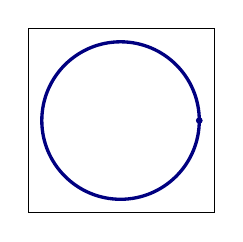
\begin{tikzpicture}[framed,scale=1,baseline=-1ex]      
            \tkzDefPoint(0,0){O} 
            \tkzDefPoint(1,0){A} 
            \tkzDrawCircle[color=penColor,very thick](O,A)
            \tkzDrawPoint[color=penColor,fill=penColor](A)
      \end{tikzpicture} We see that $b_1 = \answer[given]{1}$.
      \item 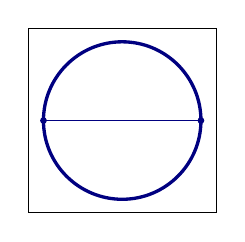
\begin{tikzpicture}[framed,scale=1,baseline=-1ex]      
            \tkzDefPoint(0,0){O} 
            \tkzDefPoint(1,0){A} 
            \tkzDefPoint(-1,0){B}
            \tkzDrawCircle[color=penColor,very thick](O,A)
            \tkzDrawPoint[color=penColor,fill=penColor](A)
            \tkzDrawPoint[color=penColor,fill=penColor](B)
            \tkzDrawSegment[color=penColor](A,B)
      \end{tikzpicture} We see that $b_2 = \answer[given]{2}$.
      \item 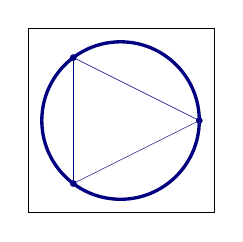
\begin{tikzpicture}[framed,scale=1,baseline=-1ex]      
            \tkzDefPoint(0,0){O} 
            \tkzDefPoint(1,0){A} 
            \tkzDefPoint(-.6,.8){B}
            \tkzDefPoint(-.6,-.8){C}
            \tkzDrawCircle[color=penColor,very thick](O,A)
            \tkzDrawPoint[color=penColor,fill=penColor](A)
            \tkzDrawPoint[color=penColor,fill=penColor](B)
            \tkzDrawPoint[color=penColor,fill=penColor](C)
            \tkzDrawSegment[color=penColor](A,B)
            \tkzDrawSegment[color=penColor](A,C)
            \tkzDrawSegment[color=penColor](B,C)
      \end{tikzpicture} We see that $b_3 = \answer[given]{4}$.
      \item 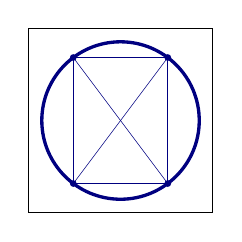
\begin{tikzpicture}[framed,scale=1,baseline=-1ex]      
            \tkzDefPoint(0,0){O} 
            \tkzDefPoint(.6,.8){A} 
            \tkzDefPoint(-.6,.8){B}
            \tkzDefPoint(-.6,-.8){C}
            \tkzDefPoint(.6,-.8){D}
            \tkzDrawCircle[color=penColor,very thick](O,A)
            \tkzDrawPoint[color=penColor,fill=penColor](A)
            \tkzDrawPoint[color=penColor,fill=penColor](B)
            \tkzDrawPoint[color=penColor,fill=penColor](C)
            \tkzDrawPoint[color=penColor,fill=penColor](D)
            \tkzDrawSegment[color=penColor](A,B)
            \tkzDrawSegment[color=penColor](A,C)
            \tkzDrawSegment[color=penColor](A,D)
            \tkzDrawSegment[color=penColor](B,C)
            \tkzDrawSegment[color=penColor](B,D)
            \tkzDrawSegment[color=penColor](C,D)
      \end{tikzpicture} We see that $b_4 = \answer[given]{8}$.
        \item 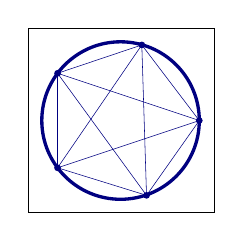
\begin{tikzpicture}[framed,scale=1,baseline=-1ex]      
            \tkzDefPoint(0,0){O} 
            \tkzDefPoint(1,0){A} 
            \tkzDefPoint(.27,.96){B}
            \tkzDefPoint(-.8,.6){C}
            \tkzDefPoint(-.8,-.6){D}
            \tkzDefPoint(.33,-.95){E}
            \tkzDrawCircle[color=penColor,very thick](O,A)
            \tkzDrawPoint[color=penColor,fill=penColor](A)
            \tkzDrawPoint[color=penColor,fill=penColor](B)
            \tkzDrawPoint[color=penColor,fill=penColor](C)
            \tkzDrawPoint[color=penColor,fill=penColor](D)
            \tkzDrawPoint[color=penColor,fill=penColor](E)
            \tkzDrawSegment[color=penColor](A,B)
            \tkzDrawSegment[color=penColor](A,C)
            \tkzDrawSegment[color=penColor](A,D)
            \tkzDrawSegment[color=penColor](A,E)
            \tkzDrawSegment[color=penColor](B,C)
            \tkzDrawSegment[color=penColor](B,D)
            \tkzDrawSegment[color=penColor](B,E)
            \tkzDrawSegment[color=penColor](C,D)
            \tkzDrawSegment[color=penColor](C,E)
            \tkzDrawSegment[color=penColor](D,E)
        \end{tikzpicture} We see that $b_5 = \answer[given]{16}$.
        \item 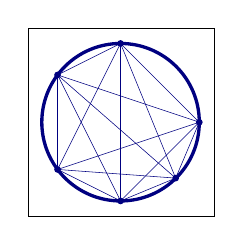
\begin{tikzpicture}[framed,scale=1,baseline=-1ex]      
            \tkzDefPoint(0,0){O} 
            \tkzDefPoint(1,0){A} 
            \tkzDefPoint(0,1){B}
            \tkzDefPoint(-.8,.6){C}
            \tkzDefPoint(-.8,-.6){D}
            \tkzDefPoint(0,-1){E}
            \tkzDefPoint(.7,-.71){F}
            \tkzDrawCircle[color=penColor,very thick](O,A)
            \tkzDrawPoint[color=penColor,fill=penColor](A)
            \tkzDrawPoint[color=penColor,fill=penColor](B)
            \tkzDrawPoint[color=penColor,fill=penColor](C)
            \tkzDrawPoint[color=penColor,fill=penColor](D)
            \tkzDrawPoint[color=penColor,fill=penColor](E)
            \tkzDrawPoint[color=penColor,fill=penColor](F)
            \tkzDrawSegment[color=penColor](A,B)
            \tkzDrawSegment[color=penColor](A,C)
            \tkzDrawSegment[color=penColor](A,D)
            \tkzDrawSegment[color=penColor](A,E)
            \tkzDrawSegment[color=penColor](A,F)
            \tkzDrawSegment[color=penColor](B,C)
            \tkzDrawSegment[color=penColor](B,D)
            \tkzDrawSegment[color=penColor](B,E)
            \tkzDrawSegment[color=penColor](B,F)
            \tkzDrawSegment[color=penColor](C,D)
            \tkzDrawSegment[color=penColor](C,E)
            \tkzDrawSegment[color=penColor](C,F)
            \tkzDrawSegment[color=penColor](D,E)
            \tkzDrawSegment[color=penColor](D,F)
            \tkzDrawSegment[color=penColor](E,F)
            \end{tikzpicture} We see that $b_6 = \answer[given]{31}$.
    \end{itemize}
    While we have made no real argument that these are the maximum
    number of regions, we believe that if the reader draws
    more pictures they will be convinced.
  \end{explanation}
\end{example}


From the two sequences we've just considered, the method of finding
a pattern is \textbf{not enough} when dealing with sequences unless
you understand exactly how the sequence was produced.  However, having
to write out all of the infinitely many terms is impossible to do!  In general, we
want to define a sequence by specifying something that will allow us to
write down any term that we want.  














\section*{Two common methods of representing the terms of a sequence}

Consider the examples presented at the beginning of the section.  While it doesn't seem likely that we can find a good pattern to describe the concentration of methane present in the atmosphere over time, there are actual patterns that can be found that predict future terms in the financial scenario as well as Fibonacci's example.

\subsection*{Explicit formulas}

Just as real-valued functions were usually expressed by a formula $f(x)$, we often encounter sequences that can be expressed by a formula $f(n)$.  When all terms $a_n$ in a sequence are described by a formula that only involves $n$ (the index), we say the sequence is defined by an \textbf{\textcolor{purple!85!blue}{explicit formula}}. It is fairly easy to work with explicit formulas.

\begin{example}
Suppose $\{a_n\}_{n=1}$ is a sequence defined by the explicit formula $a_n = 2n+3$.  Write down $a_1$, $a_2$, $a_3$, $a_4$, and $a_5$, then find $a_{500}$.

  \begin{explanation}
    By substituting $n=1, 2, 3, 4$ and $5$ into the formula above, we see
    \begin{align*}
      a_1 &= \answer[given]{5} \\ 
      a_2 &= \answer[given]{7} \\ 
      a_3 &= \answer[given]{9} \\ 
      a_4 &= \answer[given]{11} \\ 
      a_5 &= \answer[given]{13} 
    \end{align*}

Similarly, we find that $a_{500} = 2(500)+3 = \answer{1003}$.

\end{explanation}

Note that the formula $a_n = 2n+3, n \geq 1$ generates the ordered list 

\[
5,7,9,11,13, \dots ,
\]   

and there is certainly a suggested pattern. Now that we have an actual rule that gives the terms in the sequence, we can use it to verify that the pattern holds.
  
\end{example}

\begin{warning}
A common misconception is to confuse the sequence, which is the
actual ordered list of numbers, with the rule that generates it.
The sequences $\{a_n\}$ and $\{b_n\}$ given by the rules $a_n = (-1)^n$ and $b_n = \cos (\pi \cdot n)$ are different rules which give rise to the \textit{same} sequence (write out a few terms to see for yourself).  
\end{warning}



%\begin{definition}
%  Suppose $\{a_n\}_{n=1}$ and $\{b_n\}_{n=1}$ are sequences.  These
%  sequences are \dfn{equal}\index{sequence!equality} if for all
%  natural numbers $n$, we have $a_n = b_n$.
%
%  More generally, two sequences $\{a_n\}$ and $\{b_n\}$ are
%  \dfn{equal} if, after describing their terms by using the same initial index $n=N$, we have
%  \[
%  a_n = b_n \quad \text{for all $n \geq N$.}
%  \]
%  
%  This is the formal way that we say that these sequences are the same ordered list of numbers.
%\end{definition}


%Put another way, sequences are the same if they have the same set of
%valid indices, and produce the same real numbers for each of those
%indices---regardless of whether the given ``rules'' or procedures for
%computing those sequences resemble each other in any way.

\subsection*{Recursive formulas}

Sometimes, we have to know previous terms in a sequence in order to find the terms that come next.  Terms in the Fibonacci sequence stated in the introduction are easily found this way.  For instance, by taking $a_1=1$ and $a_2=1$, we find the next several terms.

\begin{align*}
a_3 = a_2+a_1 & = 1+1=2 \\
a_4 = a_3+a_2 &= 2+1 = 3 \\
a_5 = a_4+a_3 &= 3+2 = 5 \\
\end{align*}

When we have an equality that relates the next term in a sequence to the previous ones, we say that we have a \textbf{\textcolor{purple!85!blue}{recursive formula}} for the sequence.  Let's see another example.

\begin{example}
 Suppose that $\{a_n\}_{n=1}$ is a sequence defined by the formula $a_{n+1} = a_n+2$, with $a_1 = 5$.  Write down $a_2$, $a_3$, $a_4$, and $a_5$.  
 
\begin{explanation}
 Substituting in $n=2$ gives the following.
 
 \[
 a_2 = a_{1}+2 = \answer[given]{5}+2 = \answer[given]{7}
 \]
 We can now plug in $n=3$ and use the previous result for $a_2$ to find $a_3$:
  \[
 a_3 = a_{2}+2 = \answer[given]{7}+2 = \answer[given]{9}
 \]
 Continuing, we find $a_4 = \answer[given]{11}$ and $a_5 = \answer[given]{13}$.

\end{explanation}


The recursive formula generates the list 

\[
5,7,9,11,13, \dots
\]   




Note that the explicit formula $a_{n} = 2n + 3, n \geq 1$ also generates the ordered list below.

\[
5,7,9,11,13, \dots
\]   



\end{example}










\begin{example}



Note that both the explicit formula and recursive formula in the previous examples seem to generate the same list of numbers.  While writing out more and more terms suggests this is the case, \textbf{\textcolor{red!80!black}{this is not a sufficient argument}} to conclude that both rules generate the same sequence.  

In order to verify that \emph{any} term $a_n$ in the sequence whose terms are given by the formula $a_n = 2n+3$ is equal to the term $a_n$ obtained from the recursive relationship $a_{n+1}=a_n+2, a_1=5$, we first note that the first term in both sequences, $a_1$ is the same. Now, we proceed as follows.

\begin{itemize}
\item[1.] We start with the formula $a_n=2n+3$ and use this formula to write down an expression for $a_{n+1}$.
\item[2.] We verify that, after some algebra, the expression for $a_{n+1}$ satisfies the recursive relationship $a_{n+1} = a_n+2$.
\end{itemize}

Let's get started!

\begin{itemize}
\item[1.] Since $a_n=2n+3$, we have that $a_{n+1} = 2\left(\answer[given]{n+1}\right)+3$.
\item[2.] Notice that $a_n = 2n+3$, so we want to try to simplify the expression above and isolate $2n+3$, because then we can replace $2n+3$ with $a_n$. 
\end{itemize}



Letting $a_n = 2n+3$, we find the following.



\begin{align*}
a_{n+1} &= 2\left(n+1\right)+3 \\
&= 2n+5 \\
&= \left(2n+3\right) +2 \\
&= a_n+2
\end{align*}  

The term $a_n = 2n+3$ satisfies the requirement $a_{n+1}=a_n+2$, so the different looking formulas $a_n = 2n+3, n \geq 1$ and $a_{n+1}=a_n+2, a_1=5$ actually represent the same sequence.
\end{example}


%  \begin{remark}
%  The idea of ``recognizing a pattern" and using it to generate more terms for the above example can be made more mathematically explicit through the notion of \emph{mathematical induction}.  The young mathematician may hypothesize that based on the pattern in the recursive formula:
%  
%  \[
%  a_n = a_{n-1}+2, a_1 = 5
%  \]
%  
%  the explicit rule $a_n = 2n+3$ for $n \geq 1$ generates the same sequence, and may prove beyond doubt that this is indeed the case by using induction.  We leave it to the curious young mathematician to research and explore this idea further.
%  \end{remark}

\section*{Generating new sequences from other sequences}

Once we have defined a given sequence, we can make new sequences from it.  Some of the new sequences we can generate allow us to answer important questions about the original sequence.  Many of the results we obtain later on will require that we analyze sequences that we generate from others.  For now we will look at a few of these important sequences in the context of specific examples. 

\begin{example}
Suppose that $\{a_n\}_{n=1}$ is defined by the explicit formula below.

\[
a_n = 3n-1, n \geq 1
\]

Write out the first six terms in the sequence $\{a_n\}$.
\begin{explanation}
  The first few terms can be computed from the formula.
    \begin{align*}
      a_1 &= 3(1)-1=2 & 
      a_2 &= \answer[given]{5} \\ 
      a_3 &= \answer[given]{8} \\ 
      a_4 &= \answer[given]{11} \\ 
      a_5 &= \answer[given]{14}  \\ 
      a_6 &= \answer[given]{17} 
    \end{align*}
\end{explanation}


We can make new sequences from this sequence.  Here are a few examples.

\begin{question}
By noting that none of the terms in the last sequence are $0$, we
define a new sequence $\{b_n\}_{n=1}$ by the rule below.
\[
b_n = \frac{a_{n+1}}{a_n}. 
\]
Write out the first five terms in this new sequence.

\begin{explanation}
Starting with $n=1$ we find the next few terms.

\[      b_1 = \frac{a_2}{a_1} = \answer[given]{\frac{5}{2}}       \]
      
Continuing in the same way, we find:     
     \begin{align*}
      	b_2 &=  \answer[given]{\frac{8}{5}}  \\ 
	b_3 &= \answer[given]{\frac{11}{8}}  \\ 
	b_4 &= \answer[given]{\frac{14}{11}}  \\ 
	b_5 &=  \answer[given]{\frac{17}{14}}   
    \end{align*}
    
\end{explanation}
    
\end{question}

\begin{question}

Since none of the terms in the original sequence $\{a_n\}$ were
negative, we define another new sequence $\{c_n\}_{n=1}$ by the rule below.
\[
c_n = \sqrt[n]{a_n} .
\]
Write out the first five terms in this new sequence.

\begin{explanation}
Starting with $n=1$ we find  $c_1 = \sqrt[1]{a_1} = \answer[given]{2}.$
      
Continuing in the same way, we find     
     \begin{align*}
      	c_2 &=  5^{1/2}  \\ 
	c_3 &= \answer[given]{8^{1/3}}   \\ 
	c_4 &= \answer[given]{11^{1/4}}   \\ 
	c_5 &=  \answer[given]{14^{1/5}}   
    \end{align*}
    
\end{explanation}
\end{question}

\begin{question}
Define another new sequence $\{s_n\}_{n=1}$ by 

\[
s_n = \sum_{k=1}^n a_k .
\]
Write out the first five terms in this new sequence.

$\blacktriangleright$ \textbf{Note:} The notation $\sum\limits_{k=1}^n a_k$ is shorthand notation used to represent the sum $a_1+a_2+\cdots +a_n$.



\begin{explanation}
Starting with $n=1$ we find

\[      s_1 = a_1 = \answer[given]{2}.      \]
      
Continuing in the same way, we find the next few terms.    
     \begin{align*}
      	s_2 &=  a_1 +a_2 = \answer[given]{7}  \\ 
	s_3 &=  a_1 +a_2 + a_3 = \answer[given]{15}   \\ 
	s_4 &=  a_1 +a_2 +a_3 +a_4= \answer[given]{26}  \\ 
	s_5 &=  a_1 +a_2 +a_3+a_4+a_5= \answer[given]{40}    
    \end{align*}
\end{explanation}
\end{question}
\end{example}

\begin{remark} 
The following observation will be important later on, so we offer it here to give the reader a little exposure.  Note that there are two ways to compute each of the terms above.  One way is to perform the explicit addition each time, but the clever reader may notice that there is a faster way.  For instance, if we have already computed $s_3$, there is a way to use it to find $s_4$ quickly.


\begin{image}
  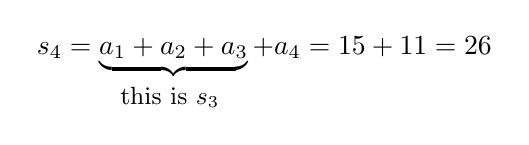
\begin{tikzpicture}
        \node at (0,0) {
          $s_4 = \underbrace{a_1+a_2+a_3} + a_4 = 15+11 =26$
        };
        \node at (-1.2,-.5) {\small{this is $s_3$}};
      \end{tikzpicture}
  \end{image}

Of course, there is a more general observation.

\begin{image}
  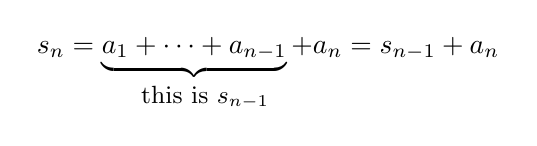
\begin{tikzpicture}
        \node at (0,0) {
          $s_n = \underbrace{a_1+\cdots+a_{n-1}} + a_n = s_{n-1} + a_n$
        };
        \node at (-.8,-.5) {\small{this is $s_{n-1}$}};
      \end{tikzpicture}
  \end{image}




so that in this example, where $a_n = 3n-1$, we have a recursive formula for $\{s_n\}_{n=1}$.

\[
s_n = s_{n-1} + (3n-1), \qquad s_1 =2
\]  
It can be shown that the recursive rule $s_n = s_{n-1} + (3n-1), s_1
=2$ and the explicit formula $s_n = \frac{3n^2+n}{2} , n \geq 1$
represent the same sequence.  We leave this to the curious reader as
an exercise.    
\end{remark}

In the preceding example, there were many new sequences that we could form from a given one.  As it turns out, these particular new sequences play an important role in answering questions about the original sequence.  

















\begin{center}
\textbf{\textcolor{green!50!black}{ooooo-=-=-=-ooOoo-=-=-=-ooooo}} \\

more examples can be found by following this link\\ \link[More Examples of Sequences]{https://ximera.osu.edu/csccmathematics/precalculus1/precalculus1/sequences/examples/exampleList}

\end{center}






\end{document}
